\chapter{Realization}
\label{ch:setup}

This chapter explains how we realized every part of our project. We present the results for each part of this chapter in the chapter \ref{ch:results}.

\section{Realization of the data recording system}

In this section, we explain how we realized the data recording system. We first explain the hardware we use and how we install it. Then, we explain how we record the data and process it to get the needed data. Finally, we explain how we use the data to train our model.

\subsection{Hardware for the recordings}
To record real data that suits our baseline, we must design a system to record and save lots of data. As we had the opportunity to place it on the HEIA-FR, we decided to design a system containing an embedded system, two microphones, a camera, and an embedded system. For the hardware, we chose to ensure that the system is easily replicable and that the system is not too expensive. We use hardware available at the HEIA and Rosas. The global architecture of the system is shown in Figure \ref{fig:global_architecture}. This diagram helps us understand how each system component is connected and how to access them.

\begin{figure}[H]
    \centering
    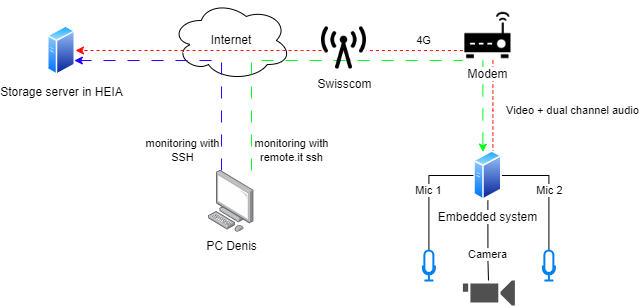
\includegraphics[width=1\textwidth]{../Images/real_data_recording_system.drawio.png}
    \caption{Global architecture}
    \label{fig:global_architecture}
\end{figure}

The HEIA-FR has a small balcony on the 4th floor with hardware installed for other projects. We use this balcony to install our system. The balcony is located on the side of a street and has a barrier on which we can attach hardware to have a good view of the street. 

To record real data that suits our baseline, we must get hardware to record and save the data. The hardware we use is the following:

\paragraph{Microphones}
We use two microphones to record the sound. We use the \textit{nsrt mk3 dev kit} from \textit{convergenceinstruments} \footnote{\url{https://convergenceinstruments.com/}} with the USB audio interface (Figure \ref{fig:nsrt_mk3_mic}). Prof. Marc-Antoine Fénart chose the microphones himself. We use two microphones to have a stereo sound recording.

\begin{figure}[H]
    \centering
    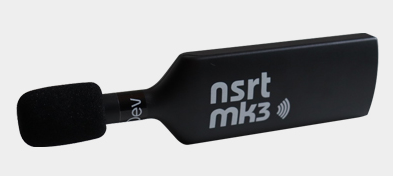
\includegraphics[width=.5\textwidth]{images/nsrt_mk3_mic.png}
    \caption{Microphone used for the recordings}
    \label{fig:nsrt_mk3_mic}
\end{figure}

\paragraph{Camera}
The camera used is a webcam from Rosas that was available at the moment of the installation. We use the \textit{C310 webcam} from \textit{logitech} \footnote{\url{https://www.logitech.fr/fr-fr/product/hd-pro-webcam-c920}} since it meets our needs (Figure \ref{fig:c310_webcam}). 

\begin{figure}[H]
    \centering
    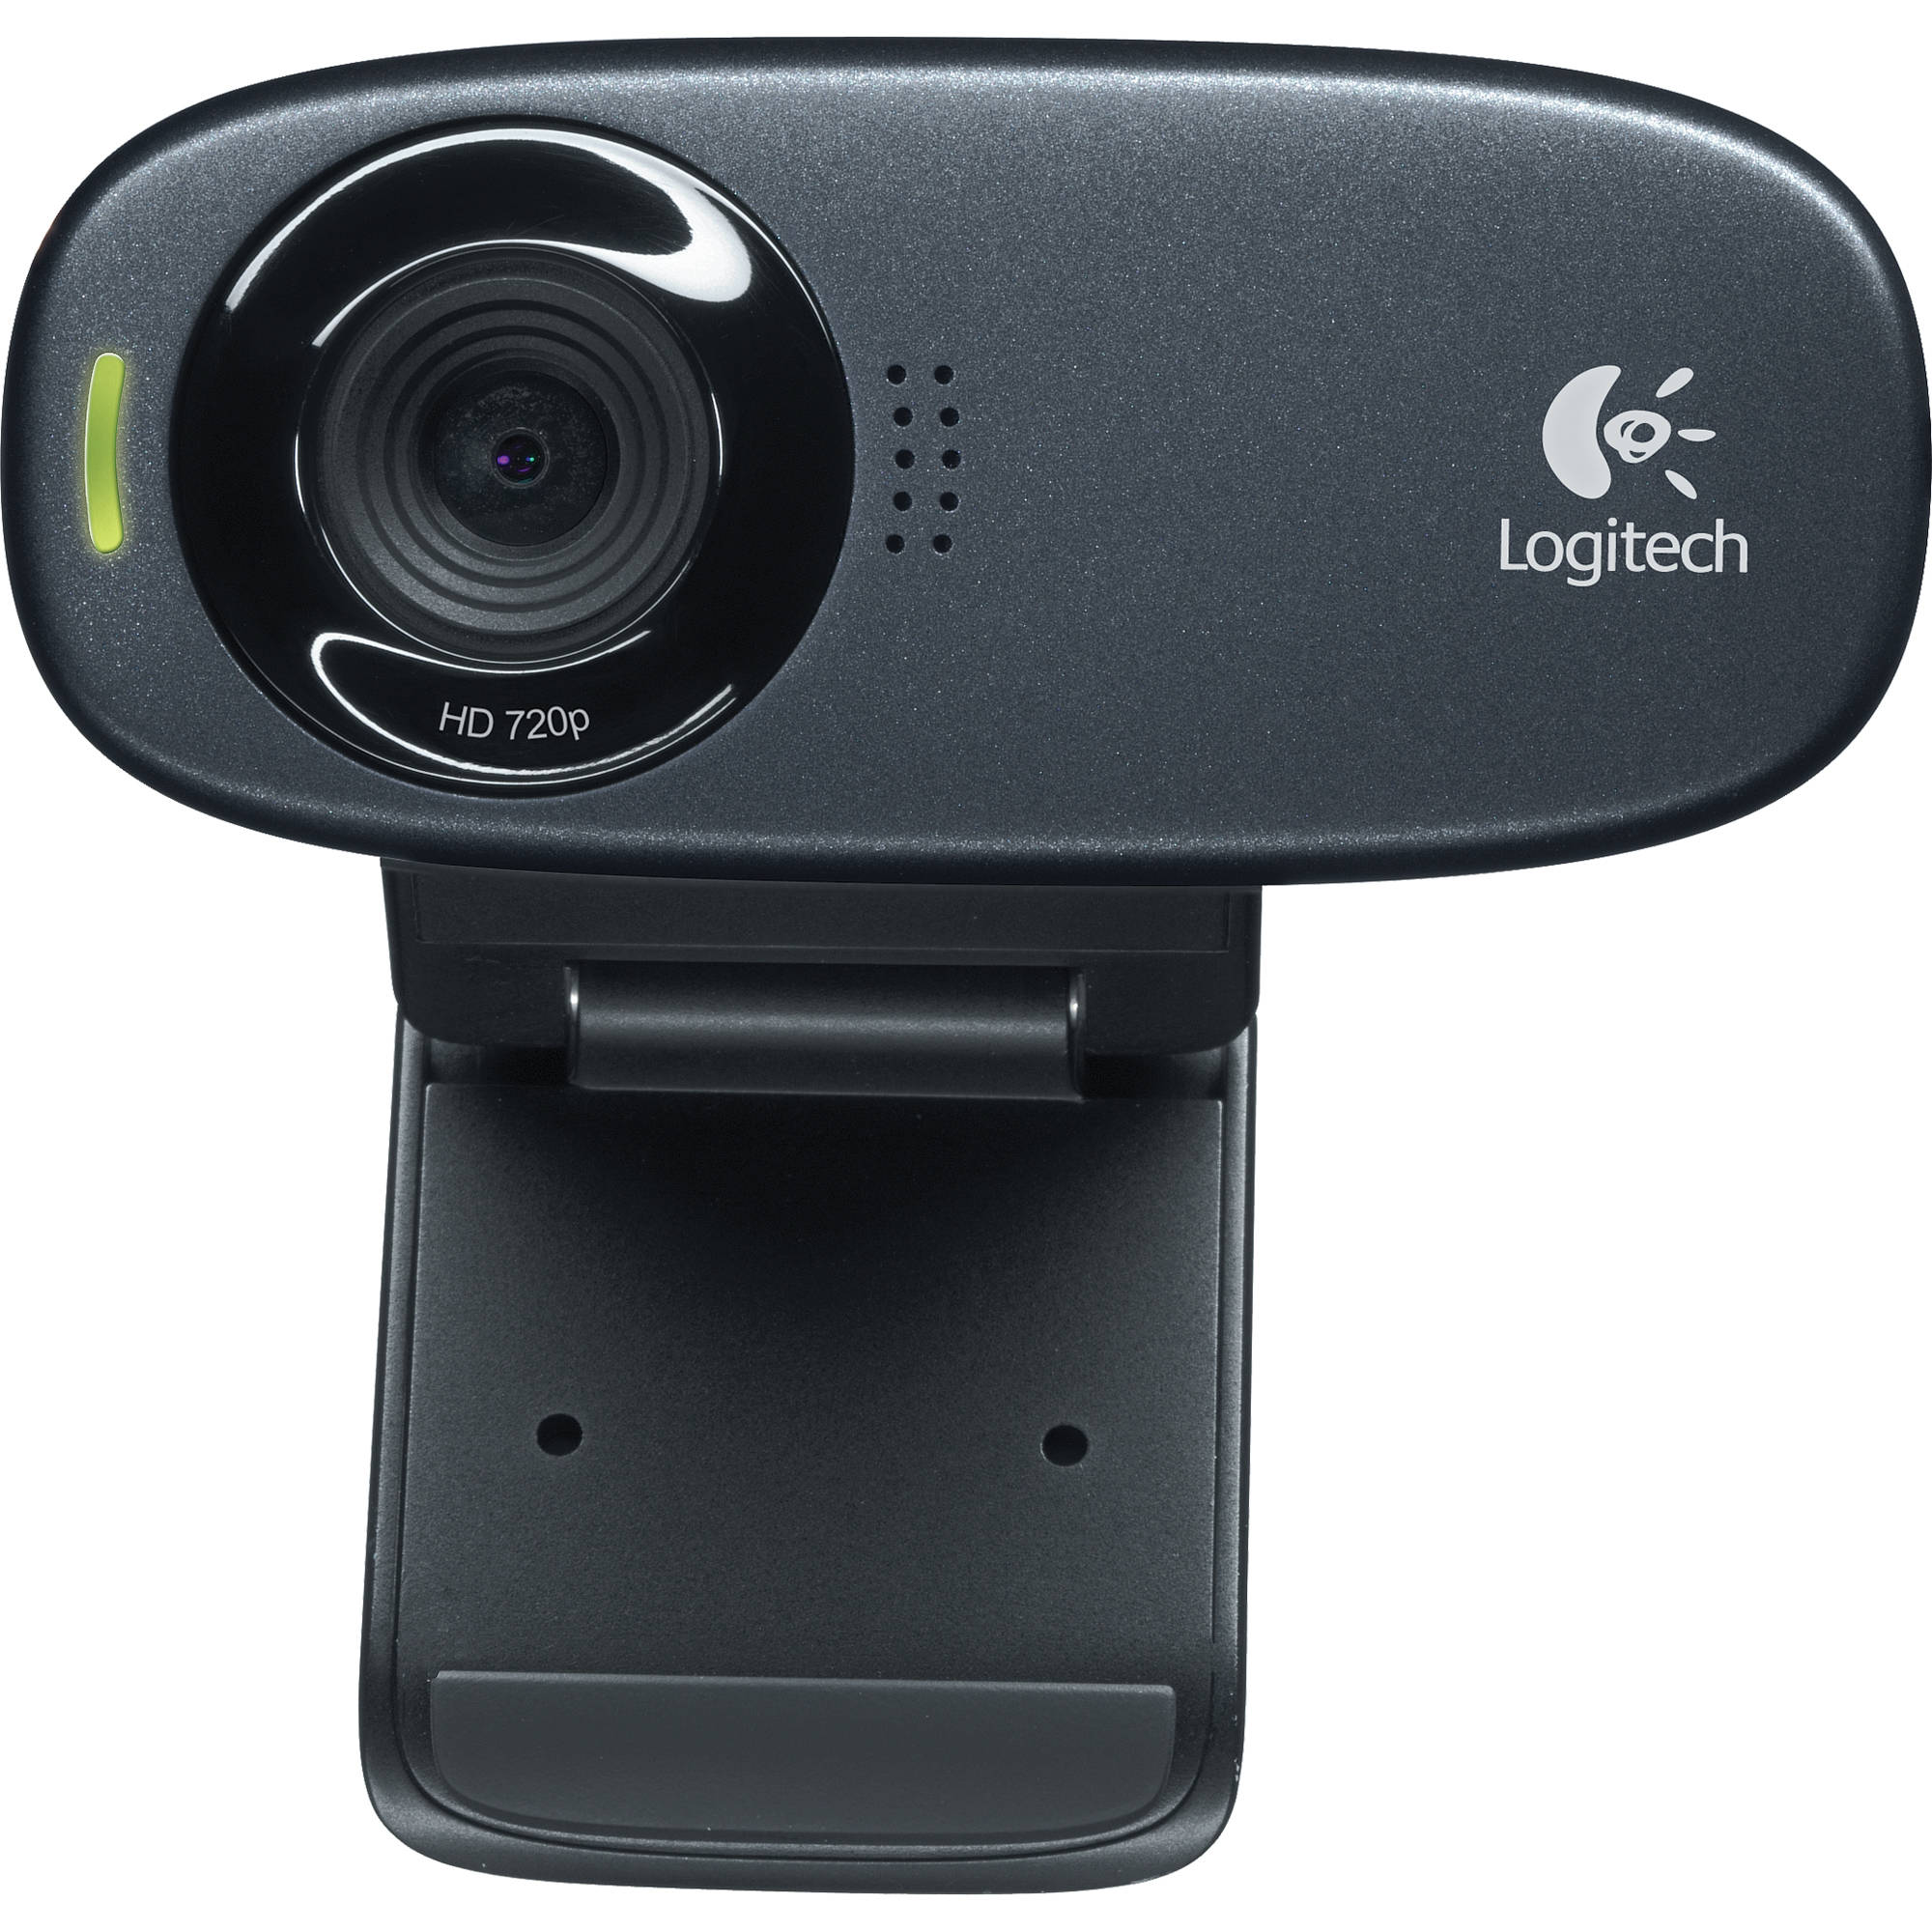
\includegraphics[width=.5\textwidth]{images/c310_webcam.png}
    \caption{Webcam used for the recordings}
    \label{fig:c310_webcam}
\end{figure}

\paragraph{Embedded system}
We use the \textit{Raspberry Pi 4} from \textit{raspberrypi} \footnote{\url{https://www.raspberrypi.org/products/raspberry-pi-4-model-b/}} as an embedded system (Figure \ref{fig:raspberry_pi_4}). We use this embedded system because it is powerful enough to run the recordings and was available at the HEIA-FR. Since our microphones and our camera have USB connectors, we needed an embedded system with at least 3 USB connectors.

\begin{figure}[H]
    \centering
    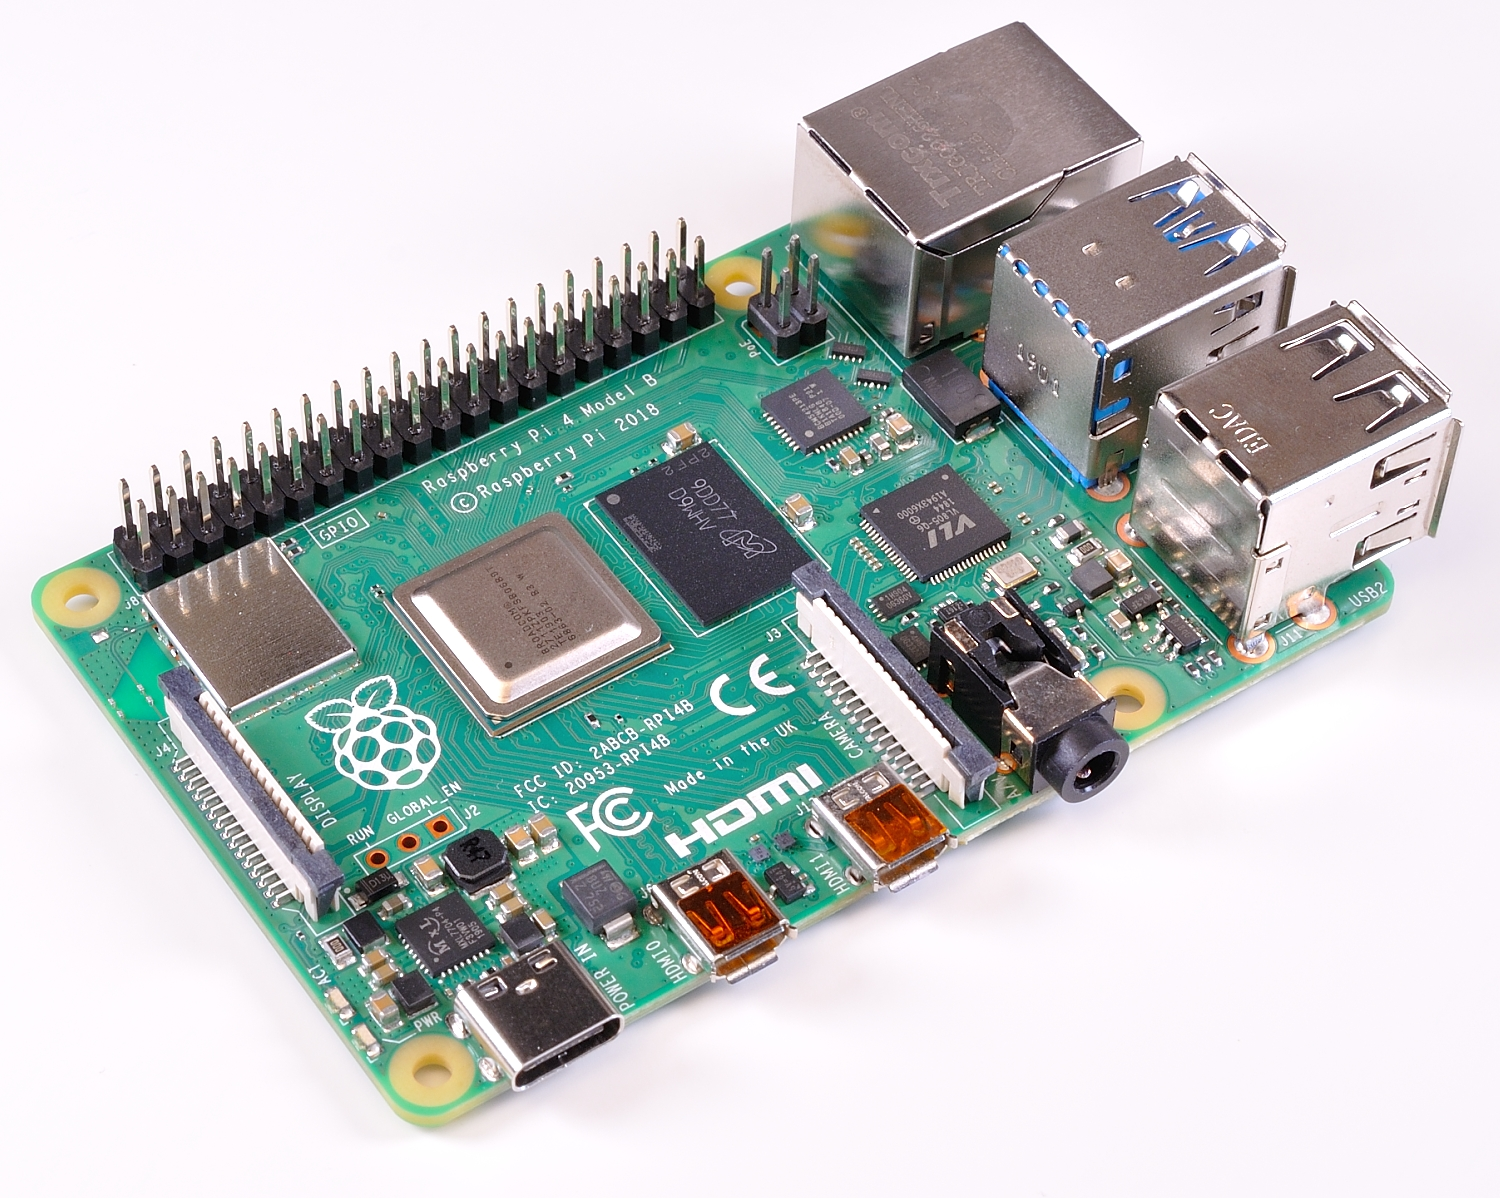
\includegraphics[width=.5\textwidth]{images/raspberry_pi_4.png}
    \caption{Raspberry Pi 4 used for the recordings}
    \label{fig:raspberry_pi_4}
\end{figure}

\paragraph{Storage}

We asked the HEIA-FR for a storage server in the school to upload the data. They lend us a server with two terabyte of storage accessible from the school network and from the internet.

\paragraph{Data transmission}

Since there is no network cable on the HEIA-FR's balcony, we use a 4G modem lent by the HEIA-FR to transmit the data to the storage server. We use a 4G LTE N300 router from D-Link \footnote{\url{https://eu.dlink.com/}} (Figure \ref{fig:4g_lte_router}) to transmit the data. We use a SIM card from Swisscom, also lent by the school to transmit the recordings via the Internet.

\begin{figure}[H]
    \centering
    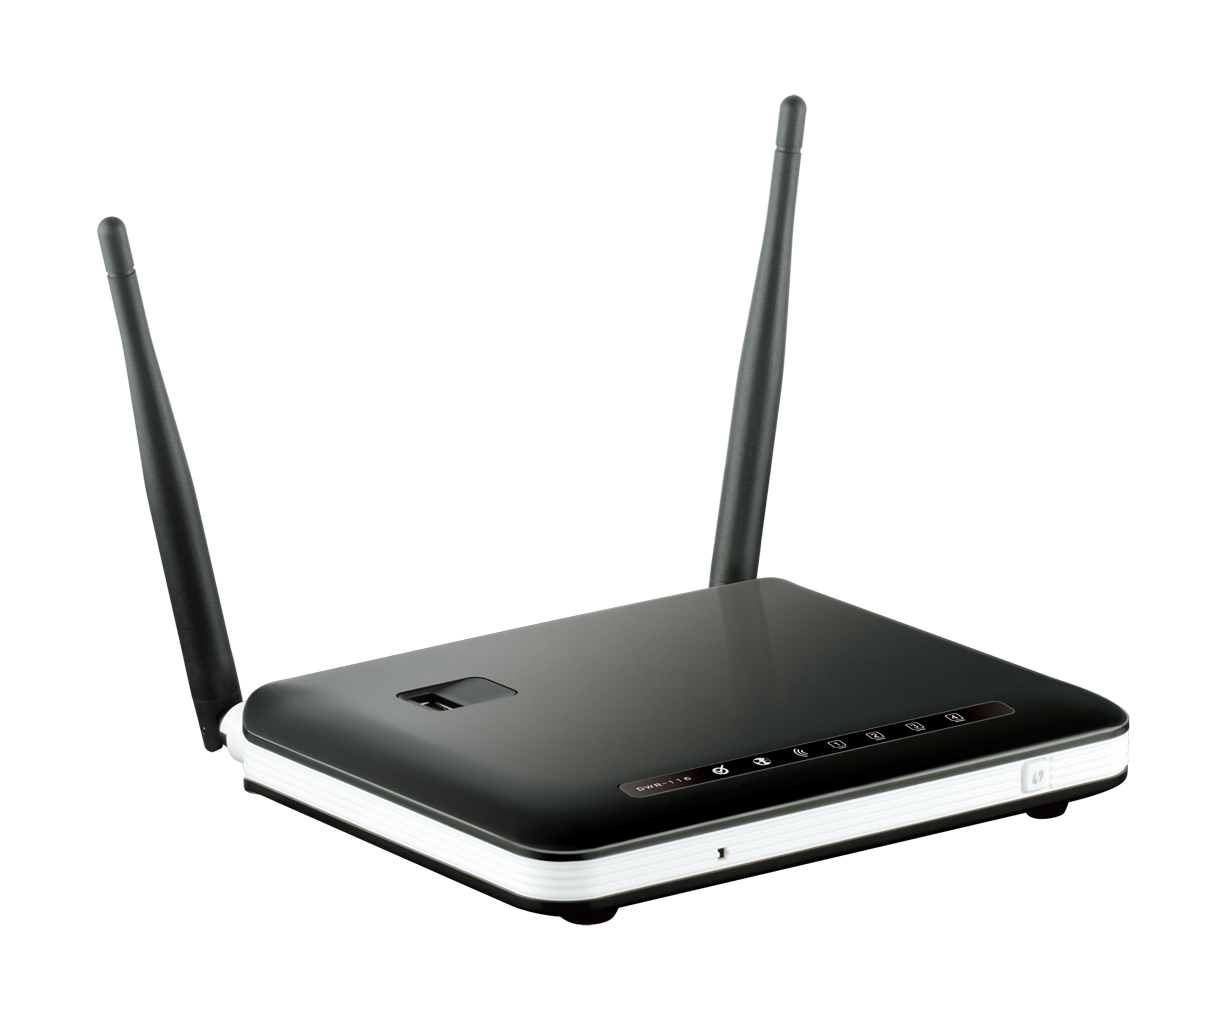
\includegraphics[width=.5\textwidth]{images/4g_lte_router.png}
    \caption{D-Link router used for the recordings}
    \label{fig:4g_lte_router}
\end{figure}

\paragraph{3D support}

To attach the microphones, we design 3D pieces with CAD software to 3D print them. We use \textit{tinkercad} to design the pieces. After the design, we give the 3D models to the mechanics at ROSAS to 3D print them (Figure \ref{fig:3d_pieces}).

\begin{figure}[H]
    \centering
    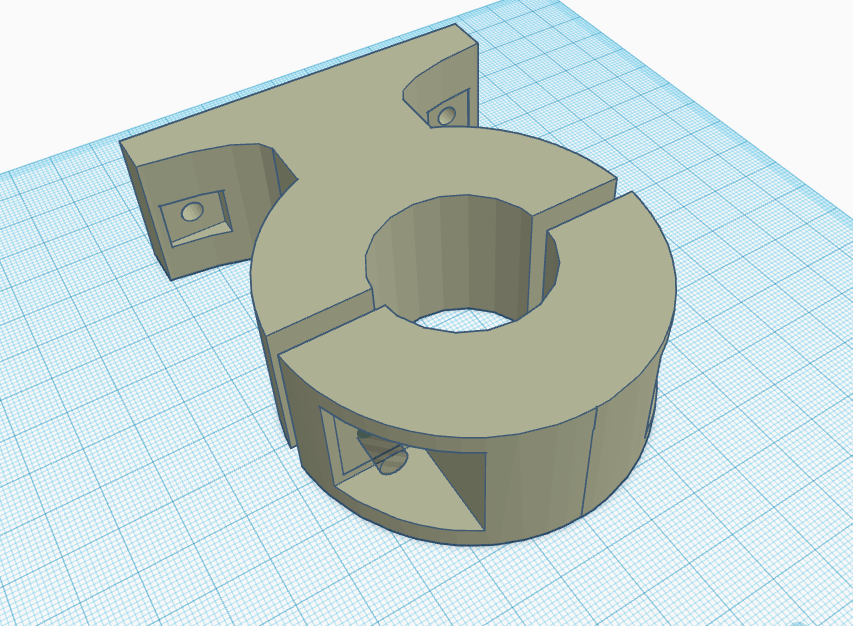
\includegraphics[width=.5\textwidth]{../Images/tinkercad_mic_support.png}
    \caption{3D pieces}
    \label{fig:3d_pieces}
\end{figure}

% TODO ajouter images
We can see the installed hardware in Figure TODO Ajouter image ! + mesure de la distance entre les micros

\subsection{Software for the recordings}

To record the data, we must have software to control the hardware. We must also have software to transmit the recorded data to the storage server. This subsection describes the software used to make the system work.

\paragraph{Operating system}

We used \textit{Raspberry Pi OS} \footnote{\url{https://www.raspberrypi.org/software/operating-systems/}} as the operating system for the Raspberry Pi because it is the official operating system and has a great community helping each other. It is based on \textit{Debian} \footnote{\url{https://www.debian.org/}} and is optimized for the Raspberry Pi. It is also easy to install and use.

\paragraph{Audio recording}

Since each microphone has its sound card, we must treat them as one sound card per microphone on the operating system. This can cause some issues if we start the recording at a slightly different time. This problem can, for example, be the case when we execute two consecutive commands, one after the other, in a script to start the microphone recording. We can use \textit{Advanced Linux Sound Architecture (ALSA)} \footnote{\url{https://www.alsa-project.org/}} to manage each sound interface and combine them into one virtual sound interface to be able to start the record from both sound cards at the same time. This can be done in a configuration file for ALSA. We used the following configuration file to combine the two sound cards into one virtual sound card:

\begin{lstlisting}
pcm.mic1 {
  type hw
  card NSRTmk3Dev
  device 0
}

pcm.mic2 {
  type hw
  card NSRTmk3Dev_1
  device 0
}

pcm.mic12 {
  type multi
  slaves.a.pcm mic1
  slaves.a.channels 1
  slaves.b.pcm mic2
  slaves.b.channels 1
  bindings.0.slave a
  bindings.0.channel 0
  bindings.1.slave b
  bindings.1.channel 0
}
\end{lstlisting}

This configuration file will create a virtual sound card called mic12 that will combine the two sound cards: \textit{mic1} and \textit{mic2}. We can then use this virtual sound card to start the recording on both sound cards simultaneously.

\paragraph{Video recording and synchronization}

We use \textit{ffmpeg} \footnote{\url{https://www.ffmpeg.org/}} to record the video and the audio synchronously. The command used to record the video and the audio is the following:

\begin{lstlisting}[language=bash]
    ffmpeg -f alsa -thread_queue_size 2048 -i plug:mic12 -f v4l2 -thread_queue_size 2048 -input_format mjpeg -video_size 600x400 -i /dev/video0 -c:a aac -map 0:a -map 1:v -segment_time 00:10:00 -f segment /mnt/videos/$current_date/output%05d.mp4
\end{lstlisting}

This command combines the video from the device \textit{/dev/video0} and the virtual sound card \textit{mic12} in a single file containing audio and video.

Before installing the system on the HEIA-FR balcony, we calculated the delay between the video and the audio by clapping in front of the webcam and the microphones. Since the delay found was inferior to 100 milliseconds and we only recorded two seconds of video to provide ground truth, we admitted it was negligible for the dataset annotation task.

\paragraph{Raspberry Pi access for administration}

We used a server from the HEIA-FR to store the data. We can access the server through OpenSSH on the local network of the HEIA-FR.

Since we don't want to go to the HEIA-FR every time we want to access the Raspberry Pi, and we don't want to have ports open on the internet, we use \textit{remote.it} \footnote{\url{https://remote.it/}} to access the Raspberry Pi remotely. \textit{Remote.it} is a service that allows us to access the Raspberry Pi remotely without opening ports on the internet. It creates a VPN between the Raspberry Pi and the \textit{remote.it} server and gives us the VPN address on the \textit{remote.it} web application. We can then access the Raspberry Pi through the VPN.


\paragraph{Data transmission}

Since the data we transmit could be sensitive, we transferred it using a secure file transfer protocol. SFTP is a network protocol that provides file access, file transfer, and file management functionalities over a secure channel. We used \textit{OpenSSH} \footnote{\url{https://www.openssh.com/}} to transfer the data. OpenSSH is a suite of secure networking utilities based on the Secure Shell (SSH) protocol. OpenSSH encrypts all traffic (including passwords) to eliminate eavesdropping, connection hijacking, and other attacks. To transfer the data, we mounted the storage server as a local drive on the Raspberry Pi by using the following command:

\begin{lstlisting}[language=bash]
    sshfs drosset@proxy51.rt3.io:/home/drosset/workspace/videos /mnt/videos -p 33838
\end{lstlisting}

This command will ask for a password to connect to the server and provide us with a local drive on the Raspberry Pi that is connected to the server. We can then use this local drive to store the data directly on the storage server.

\section{Dataset creation}

For most of the dataset management, we used Python. Python is a programming language that gives us many dataset management tools. We used Python to split the recordings into smaller files, annotate the dataset, and manage the folders.

Once we set up the hardware and the software allows us to record the vehicles on the street, we can build a dataset. The recordings of the vehicles contain audio and video in mp4 files of ten minutes each. We must split the recordings into smaller files to get to the two seconds of length defined in section \ref{sec:vehicle_recordings}. We split the recordings into two seconds files. Since splitting a video can be time-consuming, we launch it in a subprocess to execute it concurrently on multiple files at the same time. We used the following script:

\begin{lstlisting}[language=python]
for file in files:
    subprocess.call(['ffmpeg', '-i', directory + '/' + file, '-c:v', 'libx264', '-crf', '22', '-map', '0', '-segment_time', time, '-reset_timestamps', '1', '-g', '30', '-sc_threshold', '0', '-force_key_frames', 'expr:gte(t,n_forced*'+str(time)+')', '-f', 'segment', directory[:-1]+'-2sec/' + file + '%05d.mp4'])
\end{lstlisting}

This script allows to have two seconds of video clips of the vehicles. We can then annotate the dataset.

\subsection{Dataset annotation}

A good practice when creating a dataset to classify it is to put the files in folders. Each folder represents a class. In our case, we use the classes defined in section \ref{sec:dataset_conception}: 

\begin{itemize}
    \item  \textit{left\_to\_right}: Key: \textbf{D} The vehicle goes from the left to the right of the microphone.
    \item  \textit{right\_to\_left}: Key: \textbf{A} The vehicle goes from the right to the left of the microphone.
    \item  \textit{no\_cars}: Key: \textbf{S} No vehicles pass by the microphone.
    \item  \textit{multiple\_cars}: Key: \textbf{W} Multiple vehicles pass by the microphone.
\end{itemize}

Each class has its folder. We can then annotate the dataset by moving the files to the correct folder. We developed a tool to annotate the dataset. The tool is an application that shows a 2-second video from the recordings. The user can then press a key in the application to automatically move the video to the class folder. The user can also press a "cancel" key to remove the last annotated video if the user makes a mistake. Figure \ref{fig:dataset_annotation_tool} (a) shows an example of the tool. We can see multiple vehicles in this video. The user can press the \textbf{W} key. In Figure \ref{fig:dataset_annotation_tool} (b), we see only one vehicle going from right to left. The user can then press the \textbf{D} key to save the file in the correct folder.

\begin{figure}[H]
    \centering
    \subfloat[\centering Multiple car]{{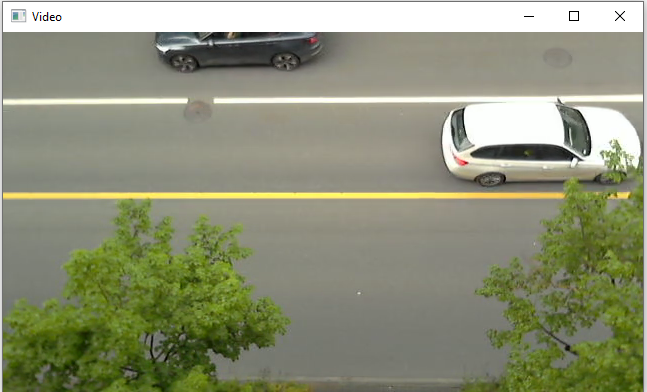
\includegraphics[width=4cm]{../Images/dataset_annotation_tool_multiple.png} }}%
    \qquad
    \subfloat[\centering Left to right]{{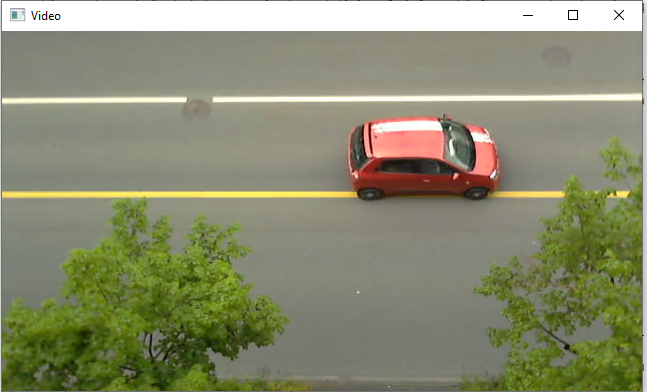
\includegraphics[width=4cm]{../Images/dataset_annotation_tool_left_to_right.png} }}%
    \caption{Dataset annotation tool}
    \label{fig:dataset_annotation_tool}
\end{figure}

Since the videos only show vehicles moving on a road, we don't need to play the video at real speed. The tool plays the video accelerated to gain time when annotating the dataset. 

\subsection{Dataset}

The annotation was done for 2037 videos and defined our baseline dataset for the project. The dataset contains 2037 videos of two seconds each. We split the dataset into four classes. The statistics for the classes are the following:

\begin{lstlisting}[language=bash]
classes:  ['left_to_right', 'multiple_cars', 'no_car', 'right_to_left']
total files:  2037
total files for class left_to_right:  513
total files for class multiple_cars:  234
total files for class no_car:  582
total files for class right_to_left:  708
\end{lstlisting}

We represent the statistics as a table in Table \ref{tab:dataset_statistics}.

\begin{table}[H]
    \centering
    \begin{tabular}{|c|c|}
        \hline
        \textbf{Class} & \textbf{Number of files} \\
        \hline
        left\_to\_right & 513 \\
        \hline
        multiple\_cars & 234 \\
        \hline
        no\_car & 582 \\
        \hline
        right\_to\_left & 708 \\
        \hline
    \end{tabular}
    \caption{Dataset statistics}
    \label{tab:dataset_statistics}
\end{table}

We made a script to shuffle the dataset and split it into training and test sets. The script's parameter defines the proportion of data in the train and test set. We use the training set to train the neural network and the test set to evaluate the neural network. The script output the number of files in each set. For example, when we run the script with a 70\% train and a 30\% test, the script gives us the following output:

\begin{lstlisting}[language=bash]
classes:  ['left_to_right', 'multiple_cars', 'no_car', 'right_to_left']
files in train:  1426
files in test:  611
total files:  2037
ratio:  0.29995090819833087
\end{lstlisting}

The script calculates the ratio to ensure that the proportion of data in the train and test set is correct.

\subsection{Dataset annotation from audio}

Since the project aims to use audio to annotate the dataset, we also create a dataset from the audio. We can use the same tool to annotate the dataset. The tool plays the audio of the video instead of the video. The user can then press the same keys to annotate the dataset. Since we use two microphones, we can play the audio in a stereo headset to have all audio channels listenable during the annotation. We can then compare the results of the dataset annotated from the audio only with the results of the neural network trained on the dataset annotated from the video. 

\section{Neural Network for Sound Source Localization}

For the neural network implementation, we use Python. Python is a popular programming language for machine learning. It is easy to use and has a lot of libraries for machine learning. The machine learning library we use is \textit{PyTorch} \footnote{\url{https://pytorch.org/}}. We use it because it is popular, open-source, and free. It also has a lot of documentation. Pytorch allows us to create neural networks in Python. It helps us create the neural network architecture, load the data, train the neural network, and test it. It uses the concept of tensor to represent the data. A tensor is a multidimensional array. To manage the arrays on the Python side, we use the \textit{numpy} \footnote{\url{https://numpy.org/}} library. We also use the \textit{matplotlib} \footnote{\url{https://matplotlib.org/}} library to plot the results. 

The shape of a tensor is a representation of the size of each of their dimension and their sizes.

\subsection{Data loading}
\label{sec:data_loading}

Once we have annotated the dataset, we can load the train set in as a matrix. The matrix contains a dimension for each sample, a dimension for each channel, and a dimension for each time step. In parallel, we keep an array with every label for each sample. We then convert the matrix to a tensor with shape ([1422, 2, 88200]). The first dimension is the number of samples in the train set (here, 1418). The second dimension is the number of channels (here, two since we recorded with two microphones). The third dimension is the number of samples (here 88200, which is two times the used sampling rate since we recorded for two seconds). 

\subsection{Data preparation}

Since we want to input spectrograms into our network, we need to convert the audio samples to spectrograms. We use the \textit{torchaudio} \footnote{\url{https://pytorch.org/audio/stable/generated/torchaudio.transforms.Spectrogram.html}} spectrogram implementation to convert each sample to a spectrogram. The spectrogram function has the following parameters:

\begin{itemize}
    \item \textbf{n\_fft}: the number of Fourier bins. We use 1000 bins.
    \item \textbf{win\_length}: the length of the window to use to compute the spectrogram. We use a window of 1000 samples.
    \item \textbf{hop\_length}: the length of the hop to use to compute the spectrogram. We use a hop of 1280 samples.
    \item \textbf{window}: the window to compute the spectrogram. We use a Hann window of 1000 samples.
    \item \textbf{normalized}: whether to normalize the spectrogram. We use a normalized spectrogram.
\end{itemize}

The spectrogram function returns a tensor with the shape [1422, 2, 501, 69]. The first two dimensions are the number of samples and channels. The third dimension is the number of frequency bins (here, 501). The fourth dimension is the number of time steps (here, 68). These parameters are the result of the spectrogram function parameters. The number of frequency bins is the number of Fourier bins divided by two plus one. The number of time steps is the number of samples minus the window length divided by the hop length plus one.

\begin{equation}
    \text{number of frequency bins} = \frac{\text{number of Fourier bins}}{2} + 1 = \frac{1000}{2} + 1 = 501
\end{equation}

\begin{equation}
    \text{number of time steps} = \frac{\text{number of samples} - \text{window length}}{\text{hop length}} + 1 = \frac{88200 - 1000}{1280} + 1 = 69
\end{equation}

After the spectrogram process, we can visualize some spectrograms. Figure \ref{fig:spectrogram} shows some spectrograms from the train set.

\begin{figure}[H]
    \centering
    \subfloat[Channel 0]{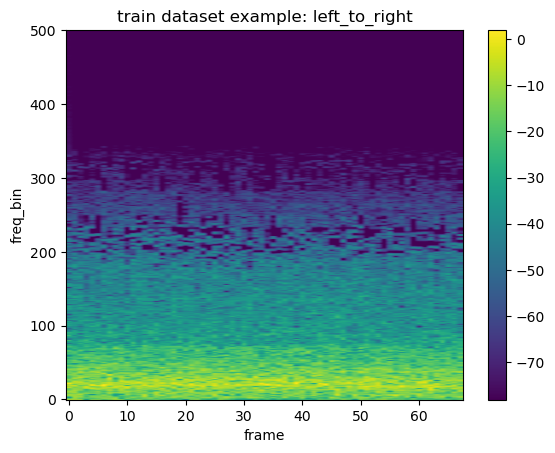
\includegraphics[width=0.4\textwidth]{images/spectrogram_left_to_right_channel0.png}}
    \qquad
    \subfloat[Channel 1]{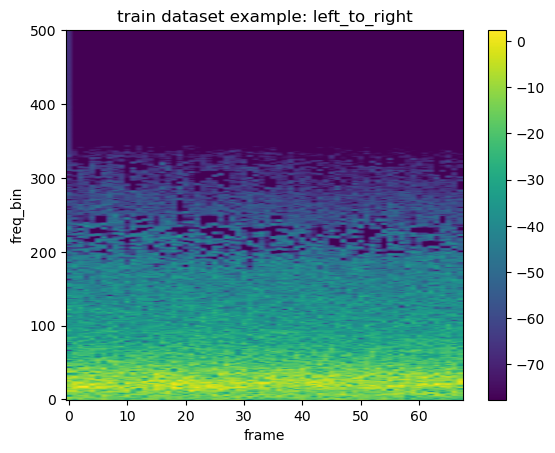
\includegraphics[width=0.4\textwidth]{images/spectrogram_left_to_right_channel1.png}}
    \caption{Spectrograms for each channel from the train set}
    \label{fig:spectrogram}
\end{figure}

And Figure \ref{fig:spectrogram_test} shows some spectrograms from the test set.

\begin{figure}[H]
    \centering
    \subfloat[Channel 0]{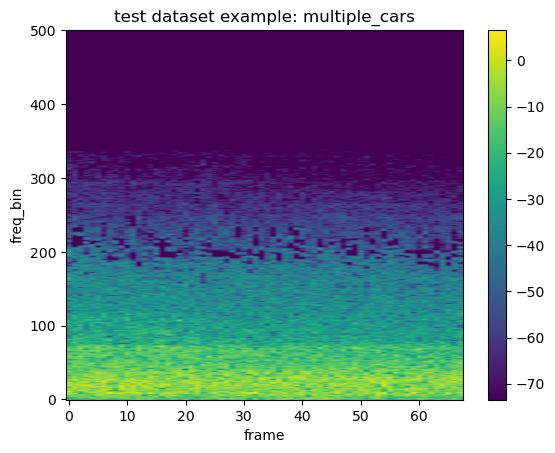
\includegraphics[width=0.4\textwidth]{images/spectrogram_multiple_cars_channel0_test.png}}
    \qquad
    \subfloat[Channel 1]{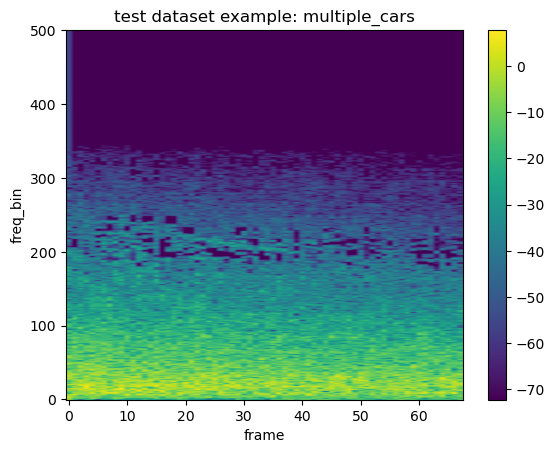
\includegraphics[width=0.4\textwidth]{images/spectrogram_multiple_cars_channel1_test.png}}
    \caption{Spectrograms for each channel from the test set}
    \label{fig:spectrogram_test}
\end{figure}

It's hard to tell the difference between the spectrograms even when they are in two different classes. That's why we use a neural network to classify them.

\subsection{Convolutional Neural Network architecture}

We use the architecture defined in section \ref{sec:cnn_design_for_ssl}. Based on the input dimension, it gives the architecture in Figure \ref{fig:cnn_architecture}. We generate this by using the \textit{sumarry} function of library \textit{torchsumarry}\footnote{\url{https://pypi.org/project/torchsummary/}}. The \textit{sumarry} function takes a neural network as input and returns the architecture of the network.

\begin{figure}[H]
    \centering
    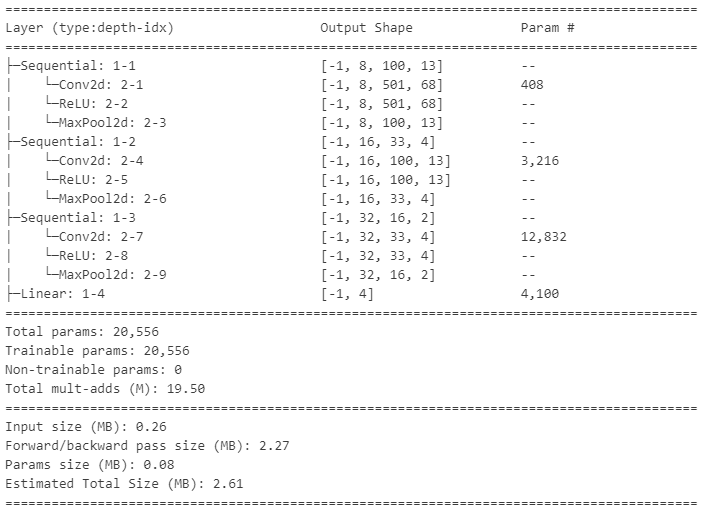
\includegraphics[width=0.5\textwidth]{images/ascii_model_architecture.png}
    \caption{Convolutional Neural Network architecture from Torchsumarry}
    \label{fig:cnn_architecture}
\end{figure}

We can better visualize the network architecture with Figure \ref{fig:cnn_architecture}. It shows us the different layers that we apply to the network. 

\begin{figure}[H]
    \centering
    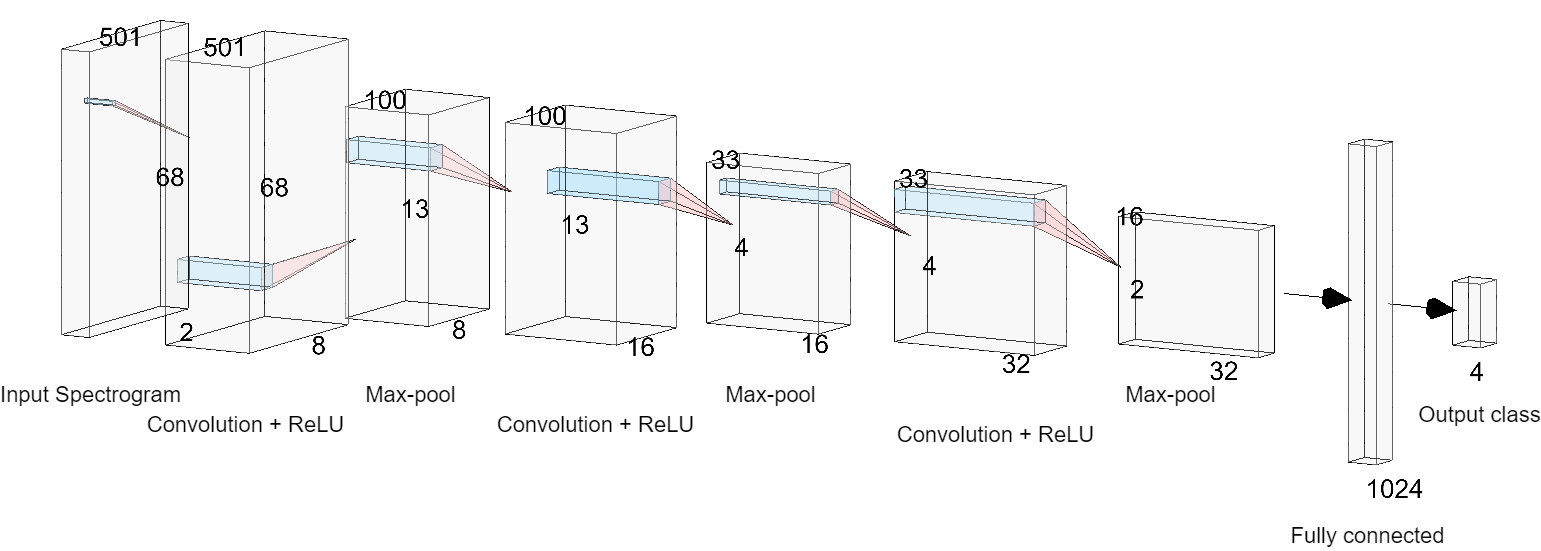
\includegraphics[width=1\textwidth]{images/tm_cnn_with_names.drawio.png}
    \caption{Convolutional Neural Network architecture}
    \label{fig:cnn_architecture}
\end{figure}

We added a dropout layer between the last layer and the output. It will help to prevent overfitting. 

Our dataset is unbalanced, so we use the weighted cross-entropy loss function. We use the pytorch implementation of the weighted cross-entropy loss function\footnote{\url{https://pytorch.org/docs/stable/generated/torch.nn.CrossEntropyLoss.html}}.

We use the Adam optimizer with a learning rate of 0.001 by using the pytorch implementation of the Adam optimizer\footnote{\url{https://pytorch.org/docs/stable/generated/torch.optim.Adam.html}}.

We also use a scheduler to reduce the learning rate when the loss function stops decreasing. We use the pytorch implementation of the ReduceLROnPlateau scheduler\footnote{\url{https://pytorch.org/docs/stable/generated/torch.optim.lr_scheduler.ReduceLROnPlateau.html}}. This will change the rate at which the optimizer will change the weights of the neural network.

\subsection{Training}
\label{sec:training}

When training, we have to define some more parameters for the training. We use the following parameters:

\begin{itemize}
    \item \textbf{batch\_size}: the number of samples to use in one batch. We use a batch size of 32.
    \item \textbf{patience}: the number of epochs to wait before reducing the learning rate. We use a patience of 3 epochs.
    \item \textbf{weight\_decay}: the weight decay. We use a weight decay of 1e-3.
\end{itemize}

We don't use the epochs count to stop the training. We use the ReduceLROnPlateau scheduler to stop the training when the learning rate is less than 1e-7. Which means that the model is nearly not learning anymore.

\subsection{Training hardware}
We used a computer with the following specifications to train the neural network:

\begin{itemize}
    \item \textbf{CPU}: Intel Core i7-10700K
    \item \textbf{GPU}: NVIDIA GeForce RTX 4070 Ti
    \item \textbf{RAM}: 32 GB
\end{itemize}

The important part of the hardware is the GPU. Since machine learning comprises many parallelizable operations, it's much faster on GPU. We use CUDA\footnote{https://developer.nvidia.com/cuda-toolkit} to use the GPU. CUDA is a parallel computing platform and application programming interface model created by Nvidia. It allows us to use the GPU to train the neural network. The Pytorch library does the CUDA integration. To use the GPU, we have to tell Pytorch to move the model and the data on the GPU by using the \textit{.to('cuda')} function.

This hardware helps us to train the neural network faster. We can train the neural network in 2 minutes on this hardware. If we don't use the GPU, the training time is multiplied by ~40. The short training time allows us to train the neural network multiple times and to try different parameters.

Once we train the network, we can use it to classify the data by giving new input data to the network. After each training, we save the model to be able to use it later.

\subsection{Training visualization}

We use \textit{Tensorboard}\footnote{\url{https://www.tensorflow.org/tensorboard}} to visualize the training. Tensorboard is a visualization toolkit for machine learning experimentation. Figure \ref{fig:tensorboard} shows the Tensorboard interface.

\begin{figure}[H]
    \centering
    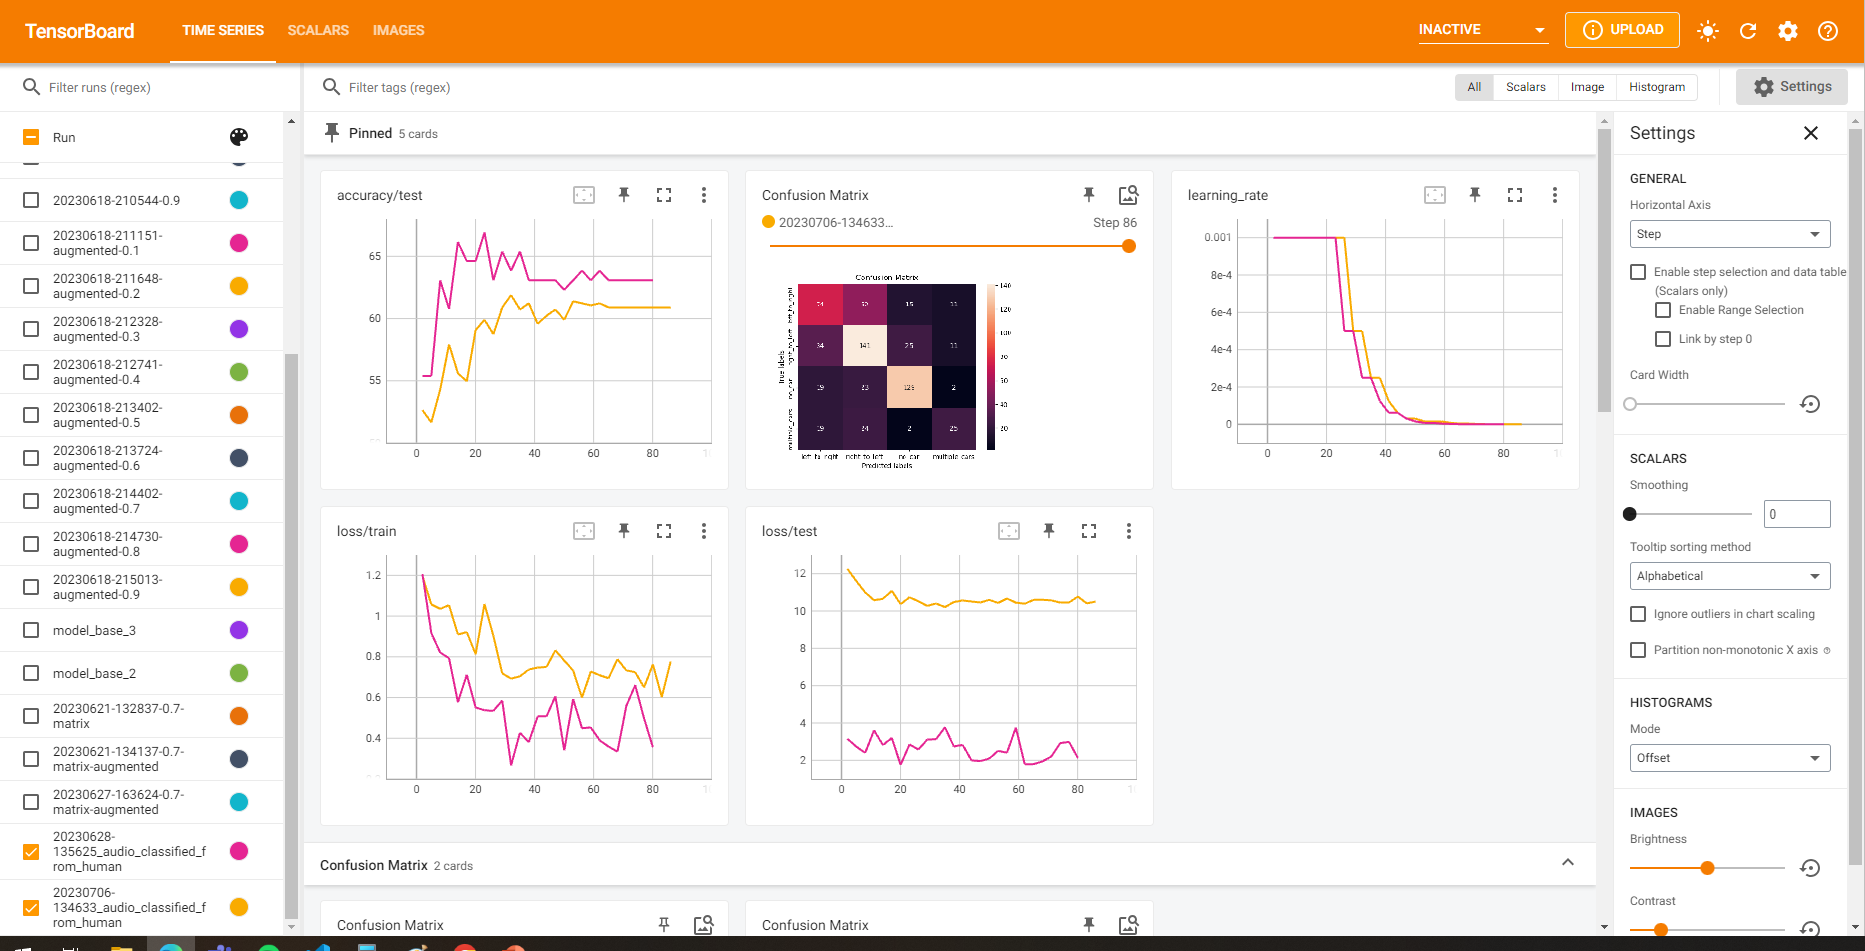
\includegraphics[width=.8\textwidth]{images/tensorboard.png}
    \caption{Tensorboard interface}
    \label{fig:tensorboard}
\end{figure}

It allows us to visualize the training loss and accuracy during the learning process. It helps to understand if we choose good hyperparameters for the training or if the neural network is learning. It also helps to compare the results between training. 

\section{Simulation model creation}

To create a dataset in simulation, we use Unity combined with the \textit{Microsoft Project Acoustic}\footnote{https://learn.microsoft.com/en-us/gaming/acoustics/what-is-acoustics} plugin. The combination of the two allows us to create a simulation of a street with vehicles passing by and to record the sound of the vehicles. We can then use the recorded sound to create a dataset. We can then use the dataset to train a neural network.

The simulation is also faster than recording the data from real life. We can generate a lot of data in a short time. The simulation is also cheaper than data recording since we only need a computer. The simulation is also more flexible than recording the data. We can change the position and comportment of every object in the simulation at any time.

\subsection{Unity}

We reproduced a street in Unity. We used the Unity Asset Store\footnote{\url{https://assetstore.unity.com/}} to get the assets to create the street. Figure \ref{fig:simulation_modelization} shows the street in Unity.

\begin{figure}[H]
    \centering
    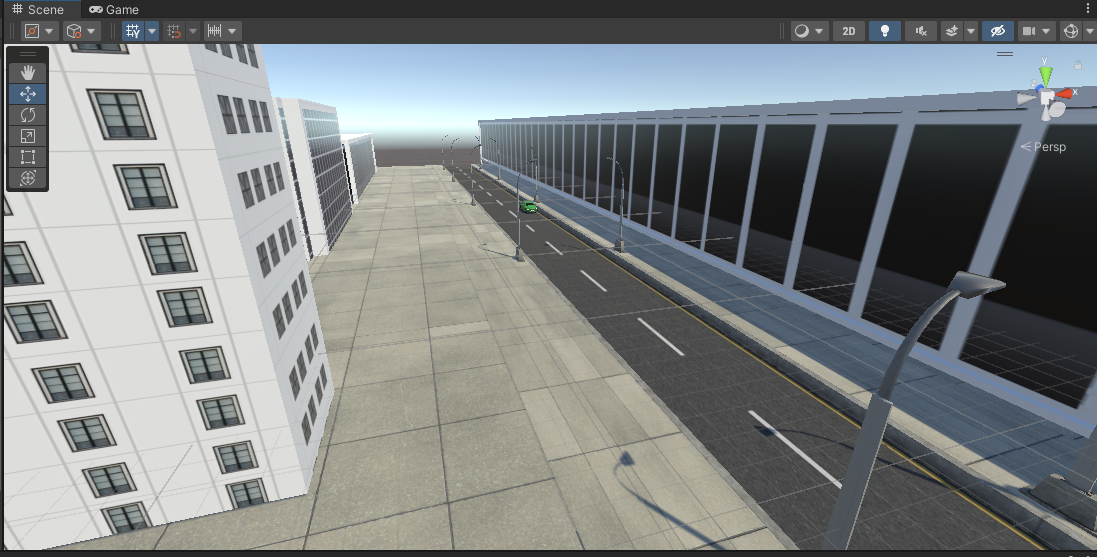
\includegraphics[width=.8\textwidth]{images/simulation_modelization.png}
    \caption{Street in Unity}
    \label{fig:simulation_modelization}
\end{figure}

\subsection{Microsoft Project Acoustic plugin}

The Microsoft Project Acoustic plugin allows us to simulate the sound propagation in the scene. We can add it in the Unity's plugin tab by following Microsoft's guide\footnote{https://learn.microsoft.com/en-us/gaming/acoustics/unity-integration}. Once it's added, we need to voxelize the scene to define which 3D surface the sound will bounce. The plugin does the voxelization and takes a short time to complete. Figure \ref{fig:simulation_voxelization} shows the voxelization of the scene. Each green square represents a voxel.

\begin{figure}[H]
    \centering
    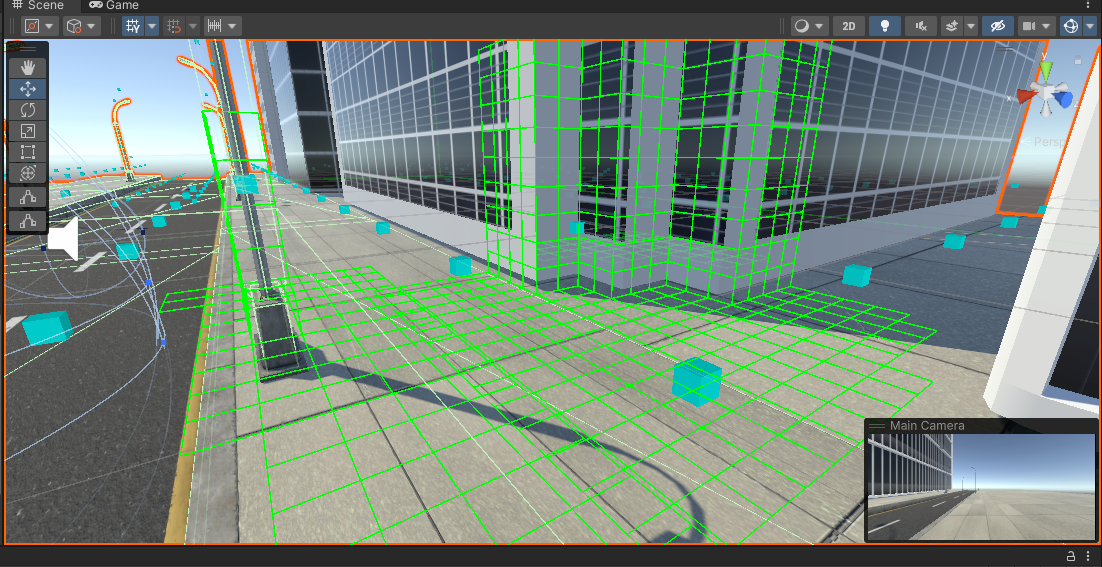
\includegraphics[width=.8\textwidth]{images/simulation_voxelization.png}
    \caption{Voxelization of the scene}
    \label{fig:simulation_voxelization}
\end{figure}

Once we finish the voxelization, we can bake the scene. Although Microsoft proposes using their Azure cloud service\footnote{https://azure.microsoft.com/fr-fr} to bake the scene, we can also bake it locally. The baking process uses docker\footnote{https://www.docker.com/} to set up the environment. The baking process takes a lot of time to complete. It took us around 2 hours to bake the scene. If we had to bake the scene multiple times, we could use the Azure cloud service to bake the scene faster.

\paragraph{Multiple channel recording in Unity}

In unity, by design, only one audio listener can be active at a time \footnote{https://docs.unity3d.com/Manual/class-AudioListener.html}. This design means that we can only record one channel at a time. To record multiple channels, we have to record each channel separately. We solve this issue by creating a script that will record each channel separately by moving the audio listener to the microphone's predetermined positions and recording the sound. We then merge the channels to create a multi-channel audio file.

\subsection{Managing sound in game engine}

In game engines, sounds travel instantly. This concept means that if we play a sound, we will hear it instantly. In real life, sound travels at 343 m/s, so we will hear it after the time it takes for the sound to travel the distance separating us from the sound origin. We have to take this into account when we create the simulation. We have to play the sound at the right time. We have to calculate the time it takes for the sound to reach the microphone. We can calculate the time with the following formula:

\begin{equation}
    t = \frac{d}{v}
\end{equation}
  
Where $t$ is the time, $d$ is the distance between the sound source and the microphone, and $v$ is the speed of sound. The speed of sound is 343 m/s. We can then play the sound after the calculated time.

Since we record each channel separately, the time difference between each channel depends on the microphone's position. We show an example of this effect in figure \ref{fig:time_delta_simulation_example} with a large distance between each microphone.

\begin{figure}[H]
    \centering
    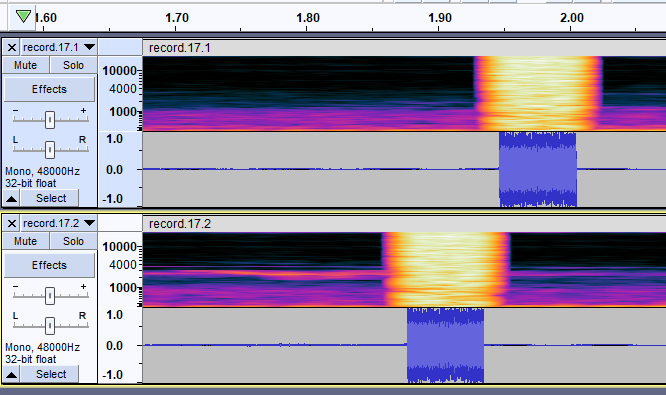
\includegraphics[width=.8\textwidth]{images/time_delta_simulation_example.png}
    \caption{Time difference between channels}
    \label{fig:time_delta_simulation_example}
\end{figure}

\paragraph{Recording the sound}

To record the sound, we use the \textit{AudioListener} component of Unity and gather each sample of the sound. We then save the samples in a wav file. We use \textit{SavWav.cs} script created by \textit{darktable} \footnote{https://gist.github.com/darktable/2317063} to create the file and save data in it.

\subsection{Creating the dataset}

We can create a folder corresponding to the class based on each class defined in section \ref{sec:simulation_concept_design}. When the simulation runs, it saves the audio file in the correct folder. Since the simulation always knows the state of the objects, we can use this information to define in which folder we need to save the audio file. This process allows us to create a dataset based on the same design as the one created with real-life data.

Once we create the dataset, we can extend the training dataset created with real-life data to improve the neural network's performance. We achieve the extension of the real-life dataset by loading the dataset the same way as the real-life dataset (in section \ref{sec:data_loading}) and extending the matrix containing the real-life dataset. We then train the model with the extended dataset by following the procedure described in section \ref{sec:training}. We generated 1267 audio files with the simulation. We then added them to the training dataset.

We detail the results of this process in section \ref{sec:augmentation_results}.

\section{Adversarial Attack}

To realize the adversarial attack, we needed to have a trained model. We used the model trained on the dataset created with real-life data. We used the \textit{Fast Gradient Signed Method} (FGSM) defined in section \ref{sec:adversarial_attack_design} as the adversarial attack design. Since we saved the model at the end of the training, we can load it and use it to create the adversarial attack.

\subsection{Adversarial example generation}

To generate adversarial examples, we need to do the equivalent of one pass of the training. The goal is to find the gradient direction that maximizes the loss. To find the sign, we can do as follow:

\begin{lstlisting}[language=Python]
    loss = criterion(model(input_tensor), label)
    loss.backward()
    perturbed_input_tensor = input_tensor + epsilon * input_tensor.grad.sign()
\end{lstlisting}

The $model(input_tensor)$ gives us the model prediction. The $label$ is the true class of the $input_tensor$. The $criterion$ is the loss function. We calculate the loss value when we call $backward()$. Once we find the loss, we can find the gradient direction by taking its sign. Once we have the direction of the gradient, we can multiply our $epsilon$ by the direction to find an image modified to maximize the loss, hence maximizing the miss-classification of the image.

The point of the FGSM on images is to get a modified image that is undetectable by the human eye. To achieve this, the $epsilon$ must be the smallest possible. To find the smallest possible $epsilon$, we can run the FGSM multiple times with an increasing $epsilon$ until we find the most efficient value of $epsilon$. This value will show the level of resistance of the model to adversarial attacks.

Once we have the $perturbed_input_tensor$, we can save it as an adversarial example.

\subsection{Audio signal reconstruction}

Since we use spectrograms, but our system records audio directly from a microphone, we need to convert the adversarial example to an audio file to attack our system. We use the \textit{friggin-lim} algorithm from \textit{pytorch} to reconstruct the audio signal from the spectrogram. Since going through a spectrogram and back to an audio signal uses multiple approximations, the reconstructed audio signal will differ from the original audio signal. We can see that the signal loses some of its information and has a smaller definition in figure \ref{fig:reconstructed_audio_signal}.

\begin{figure}[H]
    \centering
    \subfloat[Audio signal before reconstruction]{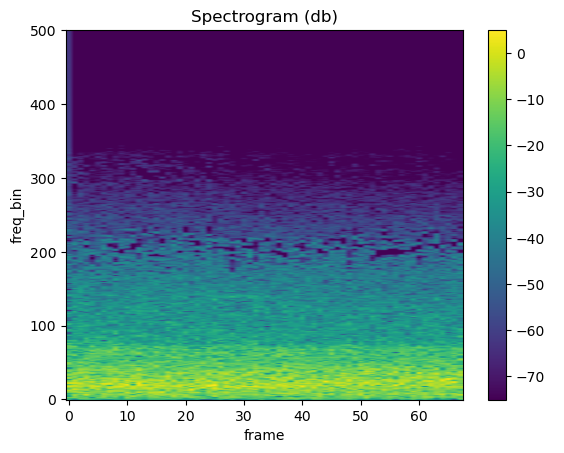
\includegraphics[width=0.4\textwidth]{images/adversarial_attack_base.png}}
    \qquad
    \subfloat[Audio signal after reconstruction]{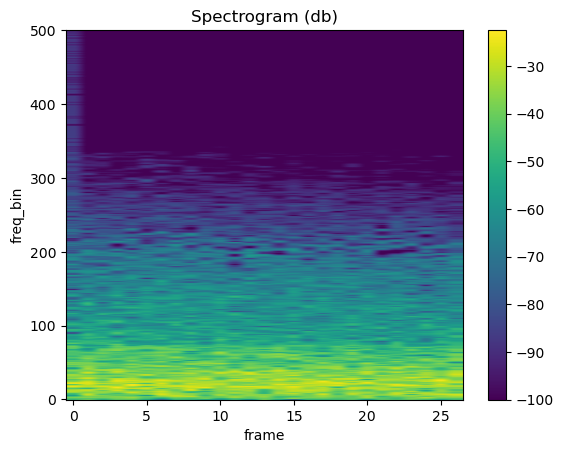
\includegraphics[width=0.4\textwidth]{images/adversarial_attack_reconstructed.png}}
    \caption{Spectrograms before and after the reconstruction}
    \label{fig:reconstructed_audio_signal}
\end{figure}

